
\documentclass[aps,prl,reprint]{revtex4-2}
\usepackage{gensymb}
\usepackage{graphicx}
\usepackage{amsmath}
\usepackage{hyperref}
\usepackage{dsfont}
\usepackage{relsize}
\usepackage{wrapfig}
\usepackage{graphicx}
\usepackage{hyperref}
\hypersetup{colorlinks=true, citecolor=blue, urlcolor=blue, linkcolor=blue}


\begin{document}

% Use the \preprint command to place your local institutional report
% number in the upper righthand corner of the title page in preprint mode.
% Multiple \preprint commands are allowed.
% Use the 'preprintnumbers' class option to override journal defaults
% to display numbers if necessary
%\preprint{}

%Title of paper
\title{RUBY}

% repeat the \author .. \affiliation  etc. as needed
% \email, \thanks, \homepage, \altaffiliation all apply to the current
% author. Explanatory text should go in the []'s, actual e-mail
% address or url should go in the {}'s for \email and \homepage.
% Please use the appropriate macro foreach each type of information

% \affiliation command applies to all authors since the last
% \affiliation command. The \affiliation command should follow the
% other information
% \affiliation can be followed by \email, \homepage, \thanks as well.
\author{Trevor Smith, Alex Storrer}
\email[]{smith.tr@northeastern.edu}
\homepage[]{https://github.com/trevorm4x/}
%\thanks{}
%\altaffiliation{}
\affiliation{Northeastern University}


\date{\today}

\begin{abstract}
	A gren laser diodde was used to excite a ruby crystal and examine its properties
	of transmission, absorption, and fluorescence. The transmission of photons with
	a wavelength of 700 nm was measured at 0.91 $\pm$ 0.05, which is higher than
	the expected value of 0.851. The absorption length for this sample was measured
	at 4.9 $\pm$ 0.1 mm. The R-line emission was measured with a wavelength of 
	693.2 $\pm$ 0.2 nm, which is slightly lower than the accepted value of 694 nm.
	The fluorescence decay constant $\tau$ was measured at 3.52 $\pm$ 0.04 ms, which
	agrees exactly with the expected value of 3.5 $\pm$ 0.5 ms.
\end{abstract}


\maketitle

% body of paper here - Use proper section commands
% References should be done using the \cite, \ref, and \label commands
\section{Introduction}
% The Introduction should contain 1 or 2 paragraphs.
% Briefly state the physics underlying the experiment
% (what is being tested and why).
In the first phase of this experiment, we will analyze the room lighting, background 
lighting, and calibrate the spcectrometer. The calibration will be done by comparing
the measured wavelength of a green laser diode to its expected wavelength of 532 nm. 
We will then block out the background light with a black cloth, and
measure the transmission and absorption spectrum of our ruby crystal sample
by measuring the intensity of a wide spectrum white light and dividing by the 
intensity of the white light after it passes through the ruby. \\

In the next phase we will investigate ruby fluorescence. Ruby fluorescence is 
key in its ability to function as a laser, where, after being excited by an incident
light source, the electrons will quickly enter a meta-stable state from which they will
more slowly exit, emitting a photon. In this lab we will be observing the wavelength of
this emittance, which corresponds to the difference in energy levels, and the lifetime
of this meta-stable state. The latter will be measured by exciting the ruby with the
same laser, but powered by a function generator in a square wave pattern. The output
of the ruby will then be collected with a photodiode and measured on an oscilloscope. 


\section{Apparatus}
% List equipment components (manufacturer, model
% numbers and brief specifications). 

The apparatus consisted of the following.
\begin{itemize}
	\item Aluminum optical breadboard with 1/4-20 tapped holes
	\item Green laser diode
	\item Spectrometer, Ocean Optics USB4000FL, OceanView software, USB cable
	\item Lens, 200mm focal length
	\item Lens, 25mm focal length
	\item Mirror in adjustable x-y mount with rotational micrometer
	\item Photodiode (PD) detector
	\item Neutral-Density (ND) optical filter
	\item Long-Pass optical filter
	\item Optical Fibers, 50 and 600 micron core
	\item Black cloth
	\item White light illuminator
	\item Ruby Crystal, Al$_2$O$_3$:Cr, approximately 0.05\% Cr
	\item Oscilloscope, Tektronix TDS1052B
	\item Signal Generator, GW Instek GFG-8216A
	\item BNC Cables and T adapter
\end{itemize}

\section{Room Light Spectrum and Calibration}

\subsection{Procedure}
% Briefly describe the experimental procedures (in your own words, but don’t overdo it)
% Discuss calibrations, etc., if required
% Include necessary equations and put them on their own line (number them, e.g. “Eq. (3)”)
% Include plots showing relevant results (label each figure, e.g. “Fig. 3”, with caption).
% Describe what you found (describe what the plot illustrates)

First, a baseline for background noise in measurements made pointed at the breadboard
was established. The OceanView software was used to tune the Scans to Average setting,
which controls the amount of time the spectrometer collects incoming photons,
to maximize the usage of the input bits of that device. This step would be performed
for each spectrometer measurement. \\

Next, the spectrometer was calibrated using the 532 nm green laser, because the
basic function of the laser will remain unchanged from its factory settings due to
the nature of how laser light is produced, while a spectrometer as a measurement
device relies on mirrors which can likely change their adjustment over time. The laser
was connected directly to the fiber-optic cable, and then to the spectrometer, which
removed any effect of the background noise.\\

Finally, the fiber-optic cable was pointed directly at the lab lights to analyze the 
spectral signature of the fluorescent lighting and other lightsources.\\

\subsection{Results}


The background measurements shown in fig. \ref{bkg} were found not to be useful, as 
the two other measurements made without the black cloth covering would be 
substantially brighter than the background noise, and the black cloth would be used 
for all future, more carefully controlled tests. This measurement may still be
relevant if any of the peaks sneak into any of the the other data they shouldn't be 
in.\\

\begin{figure}[h]
	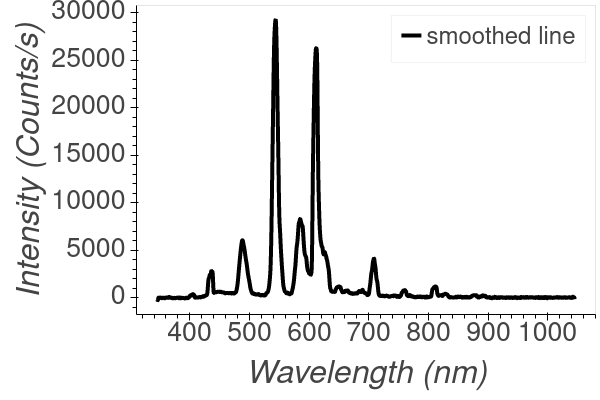
\includegraphics[width=0.4\textwidth]{../Images/l3_A_bkg.png}
	\caption{\label{bkg} Background light that reaches the test setup
	even while it is not pointed at the room.}
\end{figure}

The spectrometer measurement of the green laser was indeed found to be just over 533 nm,
meaning that all wavelength measurements using the spectrometer must be adjusted by 
1 nm. This was done proactively when loading the data from .txt file for the rest of the
lab involving the spectrometer, so all reported graphs and numbers have been corrected 
by this constant amount of 1.094 nm.

\begin{figure}[h]
	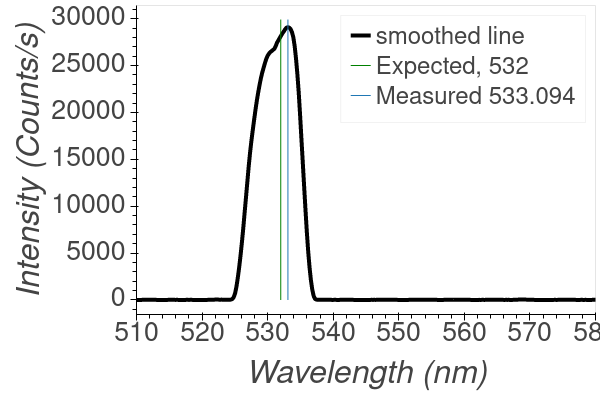
\includegraphics[width=0.4\textwidth]{../Images/l3_A_green.png}
	\caption{\label{green} The calibration of the spectrogram, performed with
	a green laser of known wavelength.}
\end{figure}

Finally the lab light spectrum was analyzed, and is given in fig.\ref{lablight}.
The 6 largest peaks were found, and their
characteristic linewidth calculated. The narrowest one was at 435.3 nm, which 
corresponds to a violet color, with a linewidth of 1.9 nm. \\

It is interesting to briefly explore why there are separate peaks. Flourescent lights
are percieved as white, but the white light source used later in the lab will have
a significantly different spectral signature in spite of being percieved in much
the same way. This is due to the nature of the photo-receptors in our eyes. The three
color-receptors in fact overlap in the wavelengths they percieve, and the brain 
compensates for these overlaps by just adding them together. This adding together of
percieved light is why, as we see in the table \ref{widths}, orange + green + yellow + 
violet + red light = white light to our eyes. Flourescent bulbs create the illusion
of white light by producing just a few different color lights, with a few different
materials. \\

\begin{figure}[h]
	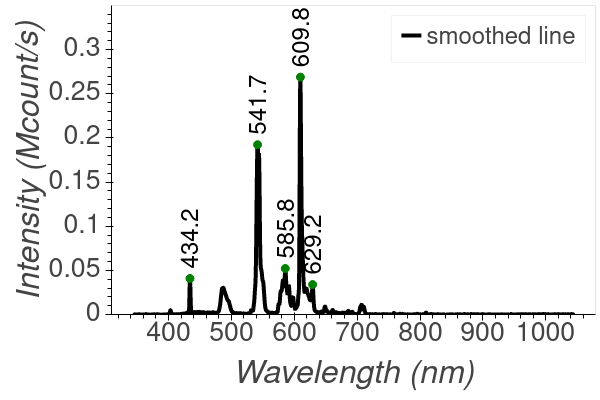
\includegraphics[width=0.4\textwidth]{../Images/l3_A_lablight.png}
	\caption{\label{lablight} The spectral signature of the laboratory, especially
	the fluorescent lighting.}
\end{figure}


\begin{table}[h]
\begin{tabular}{lrrl}
\toprule
Wavelength (nm) &  Intensity (cps) &  Linewidth (nm) &   Color \\
\hline
609.8 &     268854 &    3.3 &  Orange \\
541.7 &     192323 &    6.7 &   Green \\
585.8 &      52107 &    8.3 &  Yellow \\
434.2 &      40834 &    1.9 &  Violet \\
629.2 &      33929 &    2.2 &     Red \\\hline
\hline
\end{tabular}
\label{widths}
\end{table}

\section{Absorption Spectrum}

\subsection{Procedure}
In this phase of the lab the absorption spectrum of the ruby sample is measured. Here
we will use a white light source with a smooth output spectrum, and compare the
spectral signature of white light that does not pass through the ruby and white light
that does. The white light source was placed about 10 cm away from the FO cable 
connected to the spectrometer, and the ruby was mounted between them on a swivel to 
easily move in and out of the way of the beam. After everything was secured and aligned,
the black cloth was placed over the measurement setup to block out background noise. 
A measurement was made with and without the ruby crystal in the beam's path.
Measurements on the spectrogram were calibrated to optimize the use of its measurement
range, and the wavelengths measured were corrected by the above specified amount.


\subsection{Results}
The background noise was subtracted from each spectrum, and both are plotted in fig. \ref{ruby-no-ruby}.

\begin{figure}[h]
	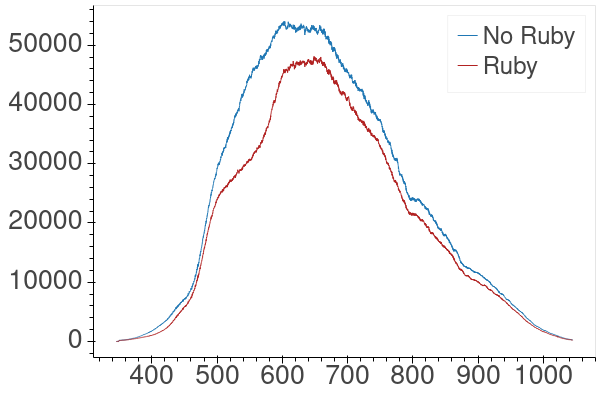
\includegraphics[width=0.4\textwidth]{../Images/l3_B_a.png}
	\caption{\label{ruby-no-ruby} A comparison of the spectral signature of the 
	white light before and after passing through the ruby crystal.}
\end{figure}

Eq. \ref{alpha} was used to calculate various facets of the expected and measured
spectral signature of the ruby. First, we examine the expected transmission at
wavelength 700 nm, assuing that $\alpha$ = 0 and using the accepted value for n, 1.7.
The exponent evaluates to 1, and thus we get $(1-R)^2$ = 0.870. This value 
corresponds to the baseline (or maybe ceiling line) for how high transmission can
be at any wavelength regardless of absorption at that wavelength, due to the portion
of the signal that will be reflected due to the mismatch in n. \\

\begin{equation}
	\mathlarger{I = I_0(1-R)^2e^{-\alpha L}}
    \label{alpha}
\end{equation}

Eq. \ref{alpha} relates the intensity of light traveling through air I to the intensity
of light traveling through a material $I_0$, a reflection coefficient R, the absorption
of the material $\alpha$, and the length of the material L.

\begin{figure}[h]
	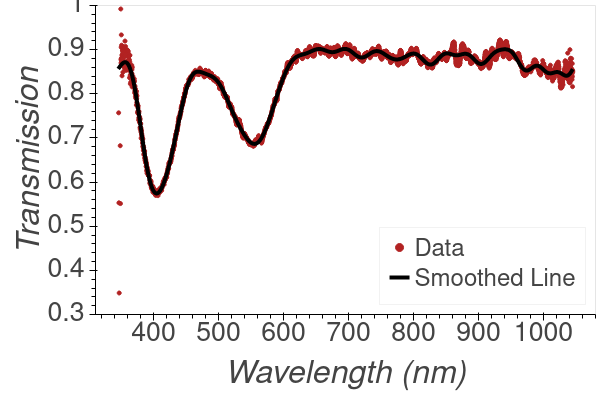
\includegraphics[width=0.4\textwidth]{../Images/l3_B_b.png}
	\caption{\label{transmission_plot} The transmission rate through a ruby sample.}
\end{figure}


The transmission spectrum, given by eq. \ref{transmission}, was computed and plotted in
\ref{transmission_plot}

\begin{equation}
	\mathlarger{T(\lambda) = I(\lambda)/I_0(\lambda)}
    \label{transmission}
\end{equation}

where $\lambda$ is the wavelength of light, and $I$ and $I_0$ are functions of
lambda that relate to the medium.

The spectrum of the absorption coefficient as a function of wavelength, 
$\alpha(\lambda)$ was computed via eq. \ref{alpha2}, which was derived from eq. 
\ref{alpha}, and plotted in fig. \ref{absorption}.

\begin{equation}
	\mathlarger{\alpha = \frac{-1}{L} \cdot ln\left(\frac{T}{(1-R)^2}\right)}
	\label{alpha2}
\end{equation}
This equation is derived from \ref{alpha} and has the same constants.

\begin{figure}[h]
	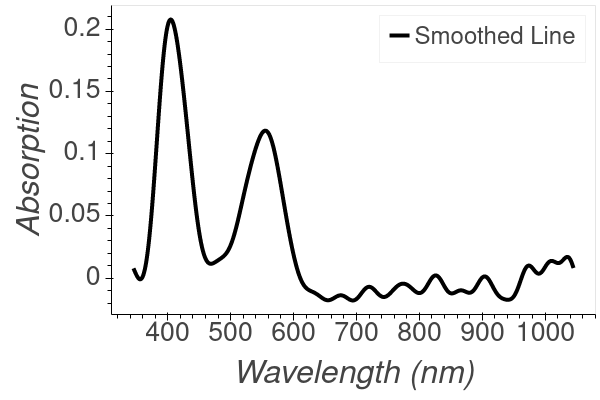
\includegraphics[width=0.4\textwidth]{../Images/l3_B_c.png}
	\caption{\label{absorption} The absorption of a ruby crystal, $\alpha(\lambda)$}
\end{figure}

The absorption peaks are centered at 400 and 550 nm, which correspond to the wavelengths
of light that the ruby absorbs. These correspond to, essentially, the other colors 
that aren't red, showing that the ruby appears red due to the red light passing through
it. The wavelength, widths and absorption lengths are given in table \ref{abs}. The
uncertainty displayed in the table was found by averaging the difference between the
raw, noisy data, and the smoothed line (smoothed using a simple lowpass filter in the
frequency domain).

\begin{table}[h]
\begin{tabular}{lrrll}
\toprule
Peak &  Wavelength (nm) &  Width (nm) &          alpha ($m^{-1}$) &        1/alpha (m) \\
\hline
1 &              404 &        56.0 &  0.206+/-0.005 &  4.9 +/- 0.1   \\
2 &              552 &        66.5 &  0.118+/-0.005 &  8.4 +/- 0.4   \\
\hline
\hline
\end{tabular}
\caption{\label{abs}}
\end{table}

\section{Ruby Fluorescence Spectrum}

\subsection{Procedure}
The optical setup was arranged to measure the emission spectrum of the ruby spectrum, 
excited by a green diode laser, shown in Fig. \ref{C}. All optical components were 
aligned by their height above the breadboard, and the 600 $\mu m$ fiberoptic cable
was mounted pointing toward the ruby crystal. The beam's intensity was reduced by
a neutral density filter, and a convex collection lens was used to focus any
output from the ruby towards the optical fiber. The lens, of focal length 25 mm, was
placed such that the image of the ruby would hit the FO with a magnification of 1,
which requires that both objects be set an equal distance from the lens. \\

\begin{equation}
	\mathlarger{\frac{1}{f} = \frac{1}{o} + \frac{1}{i}}
	\label{lens}
\end{equation}

Using the thin lens formula, where the focal length $f$ is related to object distance 
and image distance, given by \ref{lens}, the optimal distances were 
calculated to be 50 mm away from the lens.\\

\begin{figure}[h]
	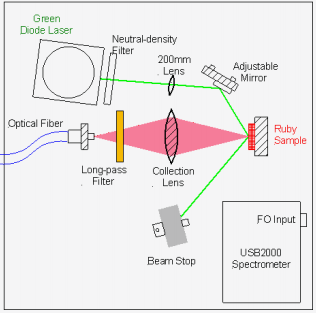
\includegraphics[width=0.4\textwidth]{../Images/l3_C.png}
	\caption{\label{C} Test setup}
\end{figure}

The setup was aligned by replacing the spectrogram at the opposite end
of the collection FO cable with a white light source, and aligning the image of the
light, as well as the green laser, directly on the ruby crystal. By replacing the 
input with an output, we can be sure that once the spectrogram is hooked up, it is
perfectly aligned to take data from the ruby crystal. After this alignment,
the spectrogram was hooked up to the FO cable and the black cloth was placed over
the apparatus. 

\subsection{Results}

The measured emission spectrum is shown in \ref{emission}. The most prominent peak,
the R-line emission of the crystal, is located at $693.2\ \pm\ 0.4\ nm$. This 
uncertainty was calculated based on 2x the measurement precision of the spectrometer.
This is given considering that, while the low-pass filter is effective at removing the 
most significant source of noise, high-frequency eletronic noise, it is still true
that different filtering techniques will yield different values, and could reasonably
correspond to a range of 5 ``markings" on the measurement device.
A brief exploration of this filtering is shown in the appendix.
This value is significant because it corresponds to the difference between the energy
level of the metastable state available in ruby crystals, and the ground state, and
with a theoretical value of 694 nm our measurement is slightly below the accepted
value. The other peak at 532 nm is due to the green laser reflecting off the surface
of the ruby.

\begin{figure}[h]
	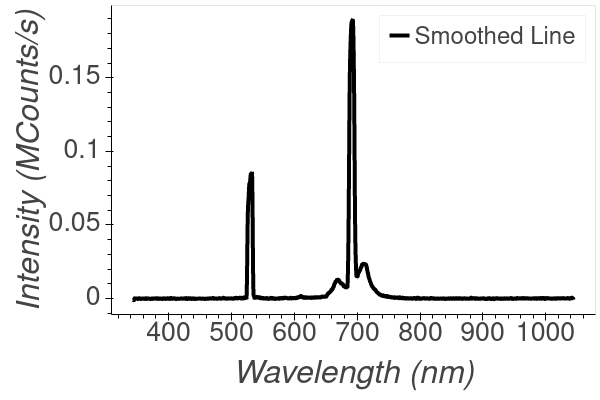
\includegraphics[width=0.4\textwidth]{../Images/l3_D_a.png}
	\caption{\label{emission} Emission of a ruby sample excited by a green laser 
	light.}
\end{figure}

\section{Fluorescence Lifetime of Ruby R-line}

\subsection{Procedure}
The optical setup was adjusted to measure the flourescence of the ruby crystal in
the time-domain. A function generator was used to produce 100 ms long laser burst,
and this signal was used to trigger an oscilloscope on the edge of the square wave. The
photodiode (PD) was connected to the FO and used to measure the fluorescence of the 
ruby and produce a signal on channel 2 of the oscilloscope. A filter was placed 
between the lens and the FO to remove the green laser light reflected from the ruby,
as discussed in the previous section. 

\subsection{Results}

\begin{figure}[h]
	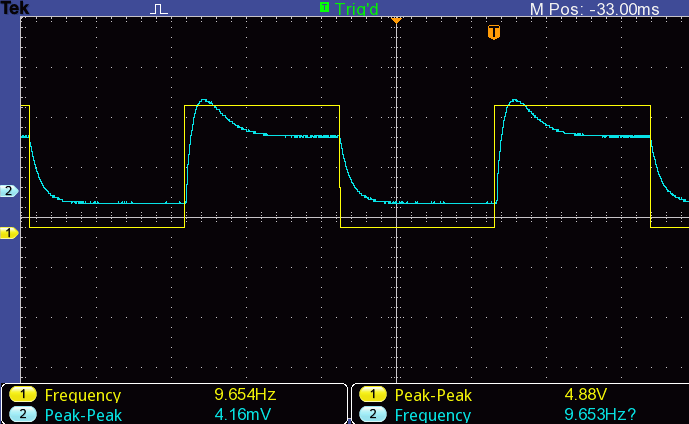
\includegraphics[width=0.4\textwidth]{../Images/l3_E_Oscilloscope.png}
	\caption{\label{scope}}
\end{figure}

Three complete periods of the PD output were captured and recorded, with the raw
data presented in fig. \ref{scope}. A inverse exponential fit (with offsets that are
not shown) was applied to each curve, beginning at the moment the laser was powered
off. After aligning the time axis such that 0 s is the moment a given laser burst ends,
and 0 mV is the asyptote of the curve, the equation is given by eq. \ref{N_0}, with
the caveat that in our measurements $N_0$ is not measured, rather a signal in mV.

\begin{equation}
	\mathlarger{N(t) = N_0e^{-t/\tau}}
	\label{N_0}
\end{equation}
This equation relates the number of electrons in an excited state, N, to the amount
of electrons originally in the excited state $N_0$ as that number decays through time
with a decay constant $\tau$. \\

The fits are shown in \ref{fits}, along with the equation given by the mean of each
variable. The lifetime of R-line ruby fluorescence, $\tau$, was calcualted at 3.52 $\pm$
0.04 ms, with the uncertainty given by the standard deviation across the three fits. 
This value overlaps with the accepted value of 3.5 $\pm$ .4 ms.

\begin{widetext}
\begin{center}
\begin{figure}[t]
	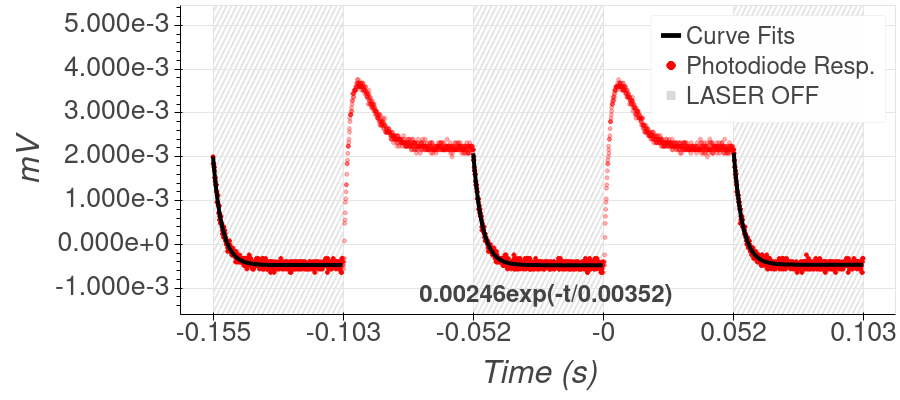
\includegraphics[width=0.8\textwidth]{../Images/l3_E.png}
	\caption{\label{fits} Three observations of the decay time of a fluorescent
	ruby sample following short laser pulses, with the average fit equation given.}
\end{figure}
\end{center}
\end{widetext}


\section{Summary}
The absorption and fluorescence of a ruby crystal was analyzed, with values for 
transmission at 700 nm, peak absorption length, R-line wavelength, and fluorescence 
lifetime calculated.\\

In the first phase of the lab, a white light source was used to produce a continuous 
curve of transmission and absorption as a function of wavelength. Using the accepted 
value for n, the index of refraction for a ruby crystal, an accepted value for the
transmission at 700 nm, assuming zero absorption, was calculated to be 0.851. The 
experimental value attained for this transmission was 0.91 $\pm$ 0.05, which is high. 
This error may stem from the shape of the white light, which was not well optimized 
towards the collection zone, or on the ruby itself. \\

An absorption curve was derived from the transmissionc curve, and the main peaks were
analyzed. While it is difficult to find an accepted value for the peak absorption
and its corresponding absorption length, $1/\alpha$, these numbers do square with
the simple observation that rubies are red, and therefore absorb the wavelengths of 
light that correspond to colors other than red. There were definitely issues with
this test setup, given the lowest values for absorption were below zero which is
not possible. It is likely that some white light was still hitting the FO input even 
after the ruby was inserted, skewing the results as though more light was getting 
through than should have been able to. It may also be that this particular sample
had a lower index of refraction than the accepted value, which would result in less
light being reflected and would also explain our observations.\\

In the next phase of the lab fluorescence was measured for its R-line wavelength and
lifetime. The measured value was 693.2 $\pm$ 0.4 nm, reasonably close to the expected
694 nm. Some of this error may be simply due to electronic noise. Interestingly, 
calibration of the spectrometer using green laser light yielded a correction of an 
about 1 nm subtraction. It may have been that this calibration was done incorrectly, as
the green light peak did not have a sharp peak, and that the measured value would be 
correct if not for miscalibration. \\

The lifetime of ruby fluorescence was measured by performing several inverse exponential
fits on the ruby emissions after short laser pulses. While the data was quite noisy
at this granularity, the fit parameters were very consistent and accurate. At 3.52 $\pm$
0.04 ms they overlapped perfectly with the accepted value of 3.5 nm. This more precise
measurement may be the result of more precise controls being possible with this setup,
and it also may be that the oscilloscope, measuring a net voltage from a photodiode,
is a more accurate measurement device than a spectrogram, which relies on measuring
very many different wavelengths and relies on precisely controlling the incoming beam.




\begin{widetext}
\begin{center}
\begin{table}[h]
\renewcommand{\arraystretch}{1.35}
\setlength{\tabcolsep}{10pt}
\caption{\label{summary}Measured and accepted values of various fluorescent properties of a ruby crystal.}
\begin{tabular}{|c|c|c|c|c|}
%\hline
\toprule
Property & Measured & Accepted & Ref. & Deviation \\
\colrule
700nm Transmission & 0.91$\pm$0.05 & 0.851 &  \cite{ruby_refraction} & 2$\sigma$ \\
\colrule
Peak Absorption Length & 4.9 $\pm$0.1 mm  & - & - & -   \\
\colrule
R-Line Wavelength & 693.2 $\pm$ 0.4 nm  & 694 nm & \cite{r-line} & -2$\sigma$ \\
%\hline
\colrule
Lifetime \tau & 3.52 $\pm$ 0.04 ms & 3.5 $\pm$ 0.5 ms & \cite{lifetime} & 0\sigma  \\
\botrule
\end{tabular}
\end{table}
\end{center}
\end{widetext}


%================================================
\begin{thebibliography}{9}
%
\bibitem{VisibleSpectrum} 
ThoughtCo, Unserstanding Visible Light \\
\href{thoughtco.com}{https://www.thoughtco.com/understand-the-visible-spectrum-608329}
%
\bibitem{ruby_refraction} 
Gem Society, Table of Refractive Indices and Double Refraction of Selected Gems \\
\href{gemsociety.org}{https://www.gemsociety.org/article/table-refractive-index-double-refraction-gems/}

\bibitem{r-line} 
Physics Open Lab, Ruby Crystal Fluorescence \\
\href{physicsopenlab.org}{https://physicsopenlab.org/2020/06/15/ruby-crystal-fluorescence/}


\bibitem{lifetime} 
SpringerLink, Ruby Crystal for Demonstrating Time- and Frequency-Domain Methods of Fluorescence Lifetime Measurements \\
\href{SpringerLink.com}{https://link.springer.com/article/10.1007/s10895-006-0123-7}
%
\end{thebibliography}


\end{document}
